\chapter{Specifikacija programske potpore}
	\section{Funkcionalni zahtjevi}
			\noindent \textbf{Dionici:}
			\begin{packed_enum}
				\item Roditelj
				\item Pedijatar
                \item Liječnik obiteljske medicine
                \item Administrator
			\end{packed_enum}
			
			\noindent \textbf{Aktori i njihovi funkcionalni zahtjevi:}
			\begin{packed_enum}
				\item  \underbar{Roditelj (inicijator) može:}
				\begin{packed_enum}
					\item registrirati se i prijaviti u sustav
                    \item vidjeti profil za sebe i svoju djecu
					\item pregledati medicinske nalaze, dijagnoze i povijesti pregleda za sebe i svoju djecu
					\item unijeti nalaz dobiven temeljem određenog pregleda ili postupka u privatnoj ustanovi
                    \item zatražiti drugo mišljenje liječnika ili pedijatra o nalazu dobivenim u privatnoj ustanovi
                    \item vidjeti zahtjeve za drugim mišljenjima koja je stvorio
				\end{packed_enum}
			
				\item  \underbar{Pedijatar (inicijator) može:}
				\begin{packed_enum}
					\item prijaviti se u sustav
                    \item prijaviti djecu po identifikatoru (OIB)
                    \item pregledati popis sve prijavljene djece i njihove kartone
					\item unijeti medicinske podatke (dijagnoze, preglede, terapije) i ažurirati te podatke
                    \item evidentirati preporuku za bolovanje za roditelja u slučaju bolesti djeteta
                    \item utvrditi bolest djeteta nakon čega se šalje ispričnica u vrtić
                    \item naručiti djecu na specijalističke preglede/postupke
                    \item dati drugo mišljenje
				\end{packed_enum}

                \item  \underbar{Liječnik obiteljske medicine (inicijator) može:}
				\begin{packed_enum}
					\item prijaviti se u sustav
                    \item pregledati i odobriti preporuke za bolovanje izdane od strane pedijatra 
					\item slati doznake za bolovanje poslodavcu roditelja
                    \item dati drugo mišljenje
                    \item naručiti pacijenta na specijalistički pregled/postupak
                    \item unositi podatke o pregledima
                    \item pristupiti medicinskim nalazima, povijesti pregleda i upitima 
				\end{packed_enum}
    
                \item  \underbar{Administrator (inicijator) može:}
				\begin{packed_enum}
                    \item prijava u sustav kao administrator
					\item pripremiti registre djece (osnovni podaci, OIB)
                    \item registrira liječnika obiteljske medicine i pedijatra
                    \item po registraciji roditelja, povezati iste s djecom (preko OIB-a)
					\item administrirati korisničke račune
                    \item ažurirati sve podatke u aplikaciji
				\end{packed_enum}

                \item  \underbar{Baza podataka (sudionik):}
				\begin{packed_enum}
                    \item pohranjuje sve podatke o korisnicima i njihovim ovlastima
				\end{packed_enum}
			\end{packed_enum}
			
			\eject 
				
			\subsection{Obrasci uporabe}
				
				%dio 1. revizije
				
				\subsubsection{Opis obrazaca uporabe}
					%Funkcionalne zahtjeve razraditi u obliku obrazaca uporabe. Ukoliko u nekom koraku može doći do odstupanja, potrebno je to odstupanje opisati i po mogućnosti ponuditi rješenje kojim bi se tijek obrasca vratio na osnovni tijek.
					

					\noindent \underbar{\textbf{UC1 - registriraj se}}
					\begin{packed_item}
	
						\item \textbf{Glavni sudionik: }korisnik
						\item  \textbf{Cilj:} stvoriti korisnički račun za pristup sustavu
						\item  \textbf{Sudionici:} baza podataka
						\item  \textbf{Preduvjet:} korisnik je otvorio početnu stranicu za registraciju u aplikaciju
						\item  \textbf{Opis osnovnog tijeka:}
						
						\item[] \begin{packed_enum}
							\item korisnik odabire opciju registriraj se
							\item sustav otvara ekran registracije
							\item korisnik unosi potrebne korisničke podatke
							\item korisnik potvrđuje unos podataka odabirom akcije potvrdi
							\item sustav provjerava i utvrđuje da je unos uspješan
							\item sustav obavještava korisnika o uspješnoj registraciji

						\end{packed_enum}
						
						\item  \textbf{Opis mogućih odstupanja:}
						
						\item[] \begin{packed_item}
							\item[4.a] Korisnik odustaje od unosa podatka (odabir akcije odustani)
							\item[] \begin{packed_enum}
								
								\item sustav zatvara trenutni ekran
								\item izvođenje scenarija je završeno
							\end{packed_enum}
							\item[5.a] Odabir već zauzetog korisničkog imena i/ili e-maila, unos korisničkih podatka u nedozvoljenom formatu
							\item[] \begin{packed_enum}
								
								\item sustav obavještava korisnika o neuspjelom upisu
								\item sustav nastavlja izvođenje u koraku 3
							\end{packed_enum}
							
						\end{packed_item}
					\end{packed_item}

                    \noindent \underbar{\textbf{UC2 - prijavi se}}
					\begin{packed_item}
	
						\item \textbf{Glavni sudionik: }korisnik
						\item  \textbf{Cilj: }dobiti pristup korisničkom sučelju
						\item  \textbf{Sudionici: }baza podataka
						\item  \textbf{Preduvjet: } izvođenje UC1
						\item  \textbf{Opis osnovnog tijeka:}
						
						\item[] \begin{packed_enum}
							\item korisniku se po upisu web adrese aplikacije, otvara početna stranica
							\item korisnik odabire akciju prijavi se
							\item sustav otvara modalni ekran prijave
							\item korisnik unosi korisničko ime i lozinku
							\item korisnik odabire akciju potvrde unosa
							\item sustav provjerava i utvrđuje da je unos uspješan
							\item korisniku se prikazuje sučelje aplikacije s korisničkim funkcijama

						\end{packed_enum}
						
						\item  \textbf{Opis mogućih odstupanja:}
						
						\item[] \begin{packed_item}
							\item[5.a] Korisnik odabire akciju Odustani
							\item[] 
							\begin{packed_enum} 
								\item sustav zatvara modalni ekran
								\item prikazuje se prethodni ekran i završava izvođenje ovog scenarija
							\end{packed_enum}
							\item[6a]  sustav provjerava i utvrđuje da unos podataka nije uspješan
							\item[] 
							\begin{packed_enum}
								\item sustav obavještava korisnika porukom na modalnom ekranu o unosu pogrešne lozinke
								\item sustav nastavlja izvođenje u koraku 4. (korisnik ispravlja unesenu lozinku i dalje scenarij ide svojim tijekom)
							\end{packed_enum}
							
						\end{packed_item}
					\end{packed_item}

                    \noindent \underbar{\textbf{UC3 - pregledaj profil djeteta}}
					\begin{packed_item}
	
						\item \textbf{Glavni sudionik: }korisnik
						\item  \textbf{Cilj:} pregledati djetetovu povijest pregleda, nalaze i dijagnoze
						\item  \textbf{Sudionici:} baza podataka
						\item  \textbf{Preduvjet:} izvođenje UC2 i UC21, korisnik ima dijete
						\item  \textbf{Opis osnovnog tijeka:}
						
						\item[] \begin{packed_enum}
		
							\item roditelj odabire opciju 'moja djeca' na početnoj stranici
							\item sustav prikazuje popis djece koja su povezana s roditeljem
							\item roditelj odabire dijete čije podatke želi pregledati
							\item sustav prikazuje početnu stranicu djetetovog profila
							\item roditelj odabire opciju 'povijest pregleda'
							\item sustav prikazuje popis svih djetetovih pregleda
							\item roditelj odabire pregled čije podatke želi pregledati
							\item sustav prikazuje podatke o odabranom pregledu
						\end{packed_enum}
						\item  \textbf{Opis mogućih odstupanja:}
						
						\item[] \begin{packed_item}
							\item[6.a] dijete nema nijedan zabilježeni pregled
							\item[] 
							\begin{packed_enum} 
								\item prikazuje se poruka 'Ne postoji nijedan zabilježeni pregled'
								\item završava izvođenje ovog scenarija
								
							\end{packed_enum}
						\end{packed_item}
					\end{packed_item}

                    
                    \noindent \underbar{\textbf{UC4 - pregledaj vlastiti profil}}
					\begin{packed_item}
	
						\item \textbf{Glavni sudionik: }korisnik
						\item  \textbf{Cilj:} pregledati vlastiti profil
						\item  \textbf{Sudionici:} baza podataka
						\item  \textbf{Preduvjet:} izvođenje UC2
						\item  \textbf{Opis osnovnog tijeka:}
						
						\item[] \begin{packed_enum}
	
							\item korisnik odabire opciju 'osobni podaci' s početne stranice
							\item sustav prikazuje osobne podatke korisnika 
			
						\end{packed_enum}
						
						
					\end{packed_item}

					\noindent \underbar{\textbf{UC5 - ažuriraj e-mail adresu poslodavca}}
					\begin{packed_item}
	
						\item \textbf{Glavni sudionik: }korisnik
						\item  \textbf{Cilj:} ažurirati e-mail adresu svog poslodavca
						\item  \textbf{Sudionici:} baza podataka
						\item  \textbf{Preduvjet:} izvođenje UC2
						\item  \textbf{Opis osnovnog tijeka:}
						
						\item[] \begin{packed_enum}
	
							\item korisnik odabire opciju 'osobni podaci' s početne stranice
							\item sustav prikazuje osobne podatke korisnika 
							\item korisnik pronalazi polje za unos e-mail adrese poslodavca
							\item korisnik odabire opciju 'uredi'
							\item sustav omogućava korisniku izmjenu/dodavanje e-mail adrese poslodavca
							\item korisnik odabire opciju 'spremi promjene'
							\item sustav provjerava i utvrđuje da je unos uspješan
							\item sustav obavještava korisnika da je unos uspješan
			
						\end{packed_enum}
						
						\item  \textbf{Opis mogućih odstupanja:}
						
						\item[] \begin{packed_item}
							\item[7.a] korisnik je unio pogrešnu e-mail adresu 
							\item[] 
							\begin{packed_enum} 
								\item prikazuje se poruka 'Pogrešan unos e-mail adrese'
								\item sustav vraća korisnika na ponovno upisivanje e-mail adrese
								\item scenarij se nastavlja od korak 6
								
							\end{packed_enum}
						\end{packed_item}
						
					\end{packed_item}

					\noindent \underbar{\textbf{UC6 - ažuriraj e-mail adresu vrtića/škole}}
					\begin{packed_item}
	
						\item \textbf{Glavni sudionik: }roditelj
						\item  \textbf{Cilj:} ažurirati e-mail adresu djetetovog vrtića/škole
						\item  \textbf{Sudionici:} baza podataka
						\item  \textbf{Preduvjet:} izvođenje UC2 i UC21
						\item  \textbf{Opis osnovnog tijeka:}
						
						\item[] \begin{packed_enum}
							\item roditelj odabire opciju 'moja djeca' s početne stranice
							\item sustav prikazuje popis djece koja su povezana s roditeljem
							\item roditelj odabire dijete čije podatke želi ažurirati
							\item sustav prikazuje osobne podatke o djetetu
							\item roditelj odabire opciju 'osobni podaci' s početne stranice
							\item sustav prikazuje osobne podatke djeteta
							\item roditelj pronalazi polje za unos e-mail adrese vrtića/škole
							\item roditelj odabire opciju 'uredi'
							\item sustav omogućava roditelju izmjenu/dodavanje e-mail adrese vrtića/škole
							\item roditelj odabire opciju 'spremi promjene'
							\item sustav provjerava i utvrđuje da je unos uspješan
							\item sustav obavještava roditelja da je unos uspješan
			
						\end{packed_enum}
						
						\item  \textbf{Opis mogućih odstupanja:}
						
						\item[] \begin{packed_item}
							\item[11.a] roditelj je unio pogrešnu e-mail adresu 
							\item[] 
							\begin{packed_enum} 
								\item prikazuje se poruka 'Pogrešan unos e-mail adrese'
								\item sustav vraća roditelja na ponovno upisivanje e-mail adrese
								\item scenarij se nastavlja od korak 10
								
							\end{packed_enum}
						\end{packed_item}
						
					\end{packed_item}


                     \noindent \underbar{\textbf{UC7 - pregledaj medicinske podatke}}
					\begin{packed_item}
	
						\item \textbf{Glavni sudionik: }korisnik
						\item  \textbf{Cilj:} pristupiti povijesti pregleda, za svaki pregled su vidljivi nalazi i dijagnoze ustanovljene na pregledu
						\item  \textbf{Sudionici:} baza podataka
						\item  \textbf{Preduvjet:} izvođenje UC2
						\item  \textbf{Opis osnovnog tijeka:}
						
						\item[] \begin{packed_enum}
	
							\item roditelj odabire opciju 'moji pregledi' s početne stranice
							\item sustav prikazuje popis svih obavljenih i zakazanih pregleda
							\item korisnik odabire pregled za koji želi vidjeti podatke
							\item sustav prikazuje podatke o odabranom pregledu
							
						\end{packed_enum}
						\item  \textbf{Opis mogućih odstupanja:}
						
						\item[] \begin{packed_item}
							\item[2.a] korisnik nema nijedan zabilježeni pregled
							\item[] 
							\begin{packed_enum} 
								\item prikazuje se poruka 'Ne postoji nijedan zabilježeni pregled'
								\item završava izvođenje ovog scenarija
								
							\end{packed_enum}
						\end{packed_item}
					\end{packed_item}

                    \noindent \underbar{\textbf{UC8 - stvori zahtjev za drugim mišljenjem}}
					\begin{packed_item}
						\item \textbf{Glavni sudionik: }korisnik
						\item  \textbf{Cilj:} zatražiti drugo mišljenja liječnika ili pedijatra o nalazu dobivenom na temelju određene usluge u privatnoj ustanovi
						\item  \textbf{Sudionici:} baza podataka
						\item  \textbf{Preduvjet:} izvođenje UC2, pacijent ima dodijeljenog liječnika ili pedijatra
						\item  \textbf{Opis osnovnog tijeka:}
						
						\item[] \begin{packed_enum}
							\item korisnik odabire opciju 'Zatraži drugo mišljenje'
							\item sustav otvara modalni okvir unosa zahtjeva za drugim mišljenjem
							\item roditelj prenosi nalaz dobiven u privatnoj ustanovi
                            \item roditelj odabire liječnika/pedijatra čije drugo mišljenje želi dobiti
							\item roditelj odabire akciju 'pošalji zahtjev'
							\item sustav provjerava i utvrđuje da je unos uspješan
							\item prikazuje se poruka 'Zahtjev uspješno poslan'
						
						\end{packed_enum}
						
						\item  \textbf{Opis mogućih odstupanja:}
						
						\item[] \begin{packed_item}
                            \item[5.a] neispravno popunjen zahtjev
                            \item[] \begin{packed_enum}
                            	\item sustav utvrđuje da je zahtjev neispravno popunjen
								\item sustav usmjerava korisnika na ponovno ispunjavanje zahtjeva za drugim mišljenjem
								\item nakon ispravnog unosa, korisnik odabire akciju 'pošalji zahtjev' te se scenarij nastavlja od koraka 6
							\end{packed_enum}
						\end{packed_item}
					\end{packed_item}


                    \noindent \underbar{\textbf{UC9 - Pregledaj zahtjev za drugim mišljenjem}}
					\begin{packed_item}
	
						\item \textbf{Glavni sudionik: }korisnik
						\item  \textbf{Cilj:} pregledati predani zahtjev za drugim mišljenjem te liječnikovu ili pedijatrovu povratnu informaciju 
						\item  \textbf{Sudionici:} baza podataka
						\item  \textbf{Preduvjet:} izvođenje UC2 i UC8
						\item  \textbf{Opis osnovnog tijeka:}
						
						\item[] \begin{packed_enum}
	
							\item korisnik odabire opciju 'moji zahtjevi' s početne stranice
							\item sustav prikazuje popis svih korisnikovih zahtjeva za drugim mišljenjem
							\item korisnik odabire zahtjev koji želi pregledati
                            \item sustav prikazuje korisnikov zahtjev za drugim mišljenjem
                            \item korisnik pregledava liječnikov odgovor na zahtjev

						\end{packed_enum}
						
						\item  \textbf{Opis mogućih odstupanja:}
						
						\item[] \begin{packed_item}
	
							\item[5.a] liječnik nije poslao svoje drugo mišljenje
							\item[] \begin{packed_enum}
								\item roditelj može vidjeti samo svoj predani zahtjev
								\item sustav prikazuje poruku 'Liječnik nije poslao svoje drugo mišljenje!' u polju za odgovor liječnika
								\item završava se izvođenje ovog scenarija 
							\end{packed_enum}
							
						\end{packed_item}
					\end{packed_item}

                    \noindent \underbar{\textbf{UC10 - prijavi pacijenta u svoju ordinaciju }}
					\begin{packed_item}
	
						\item \textbf{Glavni sudionik: }pedijatar, liječnik obiteljske medicine
						\item  \textbf{Cilj:} prijaviti pacijenta u svoju ordinaciju
						\item  \textbf{Sudionici:} baza podataka
						\item  \textbf{Preduvjet:} izvođenje UC2
						\item  \textbf{Opis osnovnog tijeka:}
						
						\item[] \begin{packed_enum}
							\item liječnik odabire opciju 'Prijavi pacijenta' s početne stranice
							\item sustav prikazuje popis pacijenata koji nemaju pridijeljenog liječnika
							\item liječnik odabire pacijenta koji postaje njegov pacijent odabirom akcije 'Odaberi pacijenta'
							\item sustav obavještava liječnika da je pacijent uspješno odabran i prijavljen u njegovu ordinaciju

						\end{packed_enum}
						
						\item  \textbf{Opis mogućih odstupanja:}
						
						\item[] \begin{packed_item}
	
							\item[2.a] ne postoji nijedan pacijent koji nema pridijeljenog liječnika
							\item[] \begin{packed_enum}
								\item sustav umjesto popisa pacijenata, prikazuje poruku 'Svi pacijenti imaju pridijeljenog liječnika'
							\end{packed_enum}
							
						\end{packed_item}
					\end{packed_item}

     
                    \noindent \underbar{\textbf{UC11 - pregledaj prijavljene pacijente i  njihove kartone }}
					\begin{packed_item}
	
						\item \textbf{Glavni sudionik: }pedijatar, liječnik obiteljske medicine
						\item  \textbf{Cilj:} pregledati popis prijavljenih pacijenata i njihovih kartona
						\item  \textbf{Sudionici:} baza podataka
						\item  \textbf{Preduvjet:} izvođenje UC2
						\item  \textbf{Opis osnovnog tijeka:}
						
						\item[] \begin{packed_enum}
	
							\item liječnik odabire opciju 'Moji pacijenti' s početne stranice
							\item sustav prikazuje popis pacijenata koji su prijavljeni u liječnikovoj ordinaciji
							\item liječnik odabire pacijenta čiji karton želi pregledati i odabire opciju 'Pregledaj karton'
							\item sustav prikazuje medicinske podatke o odabranom pacijentu
						\end{packed_enum}
						
						\item  \textbf{Opis mogućih odstupanja:}
						
						\item[] \begin{packed_item}
	
							\item[2.a] liječnik nema nijednog pacijenta
							\item[] \begin{packed_enum}
								
								\item sustav prikazuje poruku 'Nemate nijednog prijavljenog pacijenta'
								\item završava se izvođenje ovog scenarija
							\end{packed_enum}
							
						\end{packed_item}
					\end{packed_item}


                    \noindent \underbar{\textbf{UC12 - unesi pregled}}
					\begin{packed_item}
	
						\item \textbf{Glavni sudionik: }pedijatar, liječnik obiteljske medicine
						\item  \textbf{Cilj:} unijeti pregled te medicinske podatke vezane uz pregled: dijagnoza, nalaz, terapija
						\item  \textbf{Sudionici:} baza podataka
						\item  \textbf{Preduvjet:} izvođenje UC2 i UC10
						\item  \textbf{Opis osnovnog tijeka:}
						
						\item[] \begin{packed_enum}
	
							\item liječnik odabire opciju 'novi pregled' s početne stranice
							\item sustav prikazuje modalni ekran za unos pregleda
							\item liječnik odabire pacijenta iz padajućeg izbornika za kojega želi unijeti novi pregled
							\item liječnik unosi podatke o pregledu
							\item liječnik odabire opciju 'unesi pregled'
							\item sustav provjerava i utvrđuje da je unos uspješan
							\item sustav obavještava liječnika da je pregled uspješno unesen

						\end{packed_enum}

						\item  \textbf{Opis mogućih odstupanja:}
						
						\item[] \begin{packed_item}
	
							\item[6.a] liječnik je pogrešno unio podatke o pregledu
							\item[] \begin{packed_enum}
								
								\item sustav prikazuje poruku 'Neispravan unos podataka o pregledu'
								\item sustav vraća liječnika na izmjenu pogrešnih podataka o pregledu
								\item scenarij se nastavlja od koraka 5
							\end{packed_enum}
							
						\end{packed_item}
						
					\end{packed_item}

                    \noindent \underbar{\textbf{UC13 - evidentiraj preporuku za bolovanje}}
					\begin{packed_item}
	
						\item \textbf{Glavni sudionik: }pedijatar
						\item  \textbf{Cilj:} evidentirati preporuku za bolovanje roditelja u slučaju bolesti djeteta
						\item  \textbf{Sudionici:} baza podataka
						\item  \textbf{Preduvjet:} izvođenje UC2 i UC12
						\item  \textbf{Opis osnovnog tijeka:}
						
						\item[] \begin{packed_enum}
	
							\item pedijatar odabire opciju 'nova preporuka za bolovanje' s početne stranice
							\item sustav prikazuje modalni okvir za unos preporuke za bolovanje
							\item pedijatar odabire pregled na temelju kojeg je potrebna preporuka za bolovanje
							\item pedijatar unosi podatke o preporuci za bolovanje
							\item pedijatar odabire opciju 'unesi preporuku'
							\item sustav provjerava i potvrđuje da je unos uspješan
							\item sustav obavještava pedijatra da je preporuka uspješno unesena
				
						\end{packed_enum}
                    \end{packed_item}
						
                    \noindent \underbar{\textbf{UC14 - pošalji ispričnicu u vrtić/školu}}
					\begin{packed_item}
	
						\item \textbf{Glavni sudionik: }pedijatar
						\item  \textbf{Cilj:} poslati ispričnicu zbog bolesti djeteta u djetetov vrtić/školu
						\item  \textbf{Sudionici:} baza podataka
						\item  \textbf{Preduvjet:} izvođenje UC2 i UC12
						\item  \textbf{Opis osnovnog tijeka:}
						
						\item[] \begin{packed_enum}
	
							\item pedijatar odabire opciju 'Nova ispričnica' na početnoj stranici
							\item sustav prikazuje modalni ekran za unos ispričnice
							\item pedijatar odabire pregled na temelju kojega je potrebno poslati ispričnicu
                            \item pedijatar odabire opciju 'pošalji ispričnicu'
                            \item sustav provjerava i potvrđuje da je unos uspješan
                            \item sustav obavještava pedijatra da je ispričnica uspješno poslana

						\end{packed_enum}
						
						\item  \textbf{Opis mogućih odstupanja:}
						
						\item[] \begin{packed_item}
	
                            \item[5.a] pedijatar je neispravno popunio ispričnicu
							\item[] \begin{packed_enum}
								\item sustav prikazuje poruku 'Neispravan unos podataka o ispričnici'
								\item pedijatra se vraća na ponovno popunjavanje ispričnice
								\item scenarij se nastavlja od koraka 4
							\end{packed_enum}
							
						\end{packed_item}
					\end{packed_item}

     
                    \noindent \underbar{\textbf{UC15 - naruči pacijenta na specijalistički pregled/postupak }}
					\begin{packed_item}
	
						\item \textbf{Glavni sudionik: }pedijatar, liječnik obiteljske medicine
						\item  \textbf{Cilj:} naručiti pacijenta na specijalistički pregled/postupak
						\item  \textbf{Sudionici:} baza podataka
						\item  \textbf{Preduvjet:} izvođenje UC2 i UC10
						\item  \textbf{Opis osnovnog tijeka:}
						
						\item[] \begin{packed_enum}
							
							\item liječnik pregledava popis svojih pacijenata
							\item liječnik odabire pacijenta kojeg želi naručiti na specijalistički pregled/postupak
							\item liječnik stvara novi specijalistički pregled i zakaže vrijeme u budućnosti
                            \item vrijeme i lokacija se šalju pacijenti te je vidljiv pod 'Moji pregledi'

						\end{packed_enum}
					\end{packed_item}


                     \noindent \underbar{\textbf{UC16 - donesi odluku o preporuci za bolovanje}}
					\begin{packed_item}
	
						\item \textbf{Glavni sudionik: }liječnik obiteljske medicine
						\item  \textbf{Cilj:} pregledati preporuku za bolovanje roditelja izdanu od strane pedijatra
						\item  \textbf{Sudionici:} baza podataka
						\item  \textbf{Preduvjet:} izvođenje UC2 i UC13
						\item  \textbf{Opis osnovnog tijeka:}
						
						\item[] \begin{packed_enum}
							\item liječnik odabire opciju 'Preporuke za bolovanje' s početne stranice
							\item liječnik pregledava listu preporuka za bolovanje njegovim pacijentima
							\item liječnik odabire preporuku koju želi pregledati
							\item liječnik preporuku može odbiti ili prihvatiti
                            \item u slučaju da je liječnik odobrio preporuku, doznaka za bolovanje se šalje poslodavcu pacijenta

						\end{packed_enum}
					\end{packed_item}

                    
                    \noindent \underbar{\textbf{UC17 - pregledaj korisnika}}
					\begin{packed_item}
	
						\item \textbf{Glavni sudionik: }administrator
						\item  \textbf{Cilj:} pregledati registrirane korisnike
						\item  \textbf{Sudionici:} baza podataka
						\item  \textbf{Preduvjet:} izvođenje UC2
						\item  \textbf{Opis osnovnog tijeka:}
						
						\item[] \begin{packed_enum}
	
							\item administrator odabire opciju 'pregled korisnika' s početne stranice
							\item sustav prikazuje listu svih ispravno registriranih korisnika
							\item administrator odabire korisnika čije podatke želi pregledati

						\end{packed_enum}
					\end{packed_item}

                    \noindent \underbar{\textbf{UC18 - obriši korisnika}}
					\begin{packed_item}
	
						\item \textbf{Glavni sudionik: }administrator
						\item  \textbf{Cilj:} obrisati korisnika
						\item  \textbf{Sudionici:} baza podataka
						\item  \textbf{Preduvjet:} izvođenje UC2
						\item  \textbf{Opis osnovnog tijeka:}
						
						\item[] \begin{packed_enum}
							\item administrator odabire opciju 'pregled korisnika' s početne stranice
							\item sustav prikazuje listu svih ispravno registriranih korisnika
							\item administrator pronalazi željenog korisnika
							\item administrator odabire opciju 'ukloni korisnika'
							\item sustav obavještava administratora da je korisnik uspješno uklonjen
                            

						\end{packed_enum}
					\end{packed_item}

                    \noindent \underbar{\textbf{UC19 - promijeni prava pristupa}}
					\begin{packed_item}
	
						\item \textbf{Glavni sudionik: }administrator
						\item  \textbf{Cilj:} promijeniti razinu pristupa korisnika
						\item  \textbf{Sudionici:} baza podataka
						\item  \textbf{Preduvjet:} izvođenje UC2
						\item  \textbf{Opis osnovnog tijeka:}
						
						\item[] \begin{packed_enum}
							\item administrator odabire opciju 'pregled korisnika' s početne stranice
							\item sustav prikazuje listu svih ispravno registriranih korisnika
							\item administrator pronalazi željenog korisnika
							\item administrator mijenja razinu pristupa željenom korisniku odabirom opcije 'promjeni razinu pristupa'
							\item sustav obavještava administratora da je razina pristupa uspješno promijenjena
                        
						\end{packed_enum}
					\end{packed_item}
        
                    \noindent \underbar{\textbf{UC20 - administriraj registre djece i korisničke račune}}
					\begin{packed_item}
	
						\item \textbf{Glavni sudionik: }administrator
						\item  \textbf{Cilj:} upravljati registrima i korisničkim računima u sustavu
						\item  \textbf{Sudionici:} baza podataka
						\item  \textbf{Preduvjet:} izvođenje UC2
						\item  \textbf{Opis osnovnog tijeka:}
						
						\item[] \begin{packed_enum}
	
							\item administrator odabire opciju 'novi registar'
							\item sustav prikazuje modalni okvir za stvaranje djetetova registra
							\item administrator unosi podatke o korisniku: OIB, ime, prezime, adresu
							\item administrator odabire opciju 'stvori registar'
							\item sustav obavještava administratora da je registar uspješno stvoren

						\end{packed_enum}
						
					\end{packed_item}

                    \noindent \underbar{\textbf{UC21 - poveži roditelja s djetetom}}
					\begin{packed_item}
	
						\item \textbf{Glavni sudionik: }administrator
						\item  \textbf{Cilj:} povezati profil roditelja s registrom njegove djece u sustavu
						\item  \textbf{Sudionici:} baza podataka
						\item  \textbf{Preduvjet:} izvođenje UC1, UC2, UC20
						\item  \textbf{Opis osnovnog tijeka:}
						
						\item[] \begin{packed_enum}
							\item administrator odabire opciju 'pregled korisnika' s početne stranice
							\item sustav prikazuje listu svih ispravno registriranih korisnika
							\item administrator pronalazi željenog korisnika
							\item administrator odabire opciju 'poveži s djetetom'
							\item sustav prikazuje modalni okvir za povezivanje korisnika s djetetom
							\item sustav prikazuje popis registara djece koji još nisu povezani s roditeljima
							\item administrator odabire registar djeteta s kojim želi povezati roditelja
							\item administrator odabire opciju 'završi povezivanje'
							\item sustav obavještava administratora da je roditelj uspješno povezan s djetetom
						
						\end{packed_enum}
						
					\end{packed_item}
                    
        
                    \noindent \underbar{\textbf{UC22 - ažuriraj podatke u aplikaciji}}
					\begin{packed_item}
	
						\item \textbf{Glavni sudionik: }administrator
						\item  \textbf{Cilj:} ažurirati sve podatke u aplikaciji, uključujući podatke o korisnicima i njihovim ovlastima
						\item  \textbf{Sudionici:} baza podataka
						\item  \textbf{Preduvjet:} UC2
						\item  \textbf{Opis osnovnog tijeka:}
						
						\item[] \begin{packed_enum}
							\item administrator odabire opciju 'pregled korisnika' s početne stranice
							\item administrator pronalazi željenog korisnika
							\item administrator odabire opciju 'uredi'
							\item sustav prikazuje profil odabranog korisnika
							\item administrator izmjenjuje osobne podatke o korisniku i njegove medicinske podatke
							\item administrator odabire opciju spremi
							\item sustav obavještava administratora da su podaci uspješno ažurirani
						
						\end{packed_enum}
					
					\end{packed_item}

    
				\subsubsection{Dijagrami obrazaca uporabe}
					
					%Prikazati odnos aktora i obrazaca uporabe odgovarajućim UML dijagramom. Nije nužno nacrtati sve na jednom dijagramu. Modelirati po razinama apstrakcije i skupovima srodnih funkcionalnosti.
					\begin{figure}[H]
						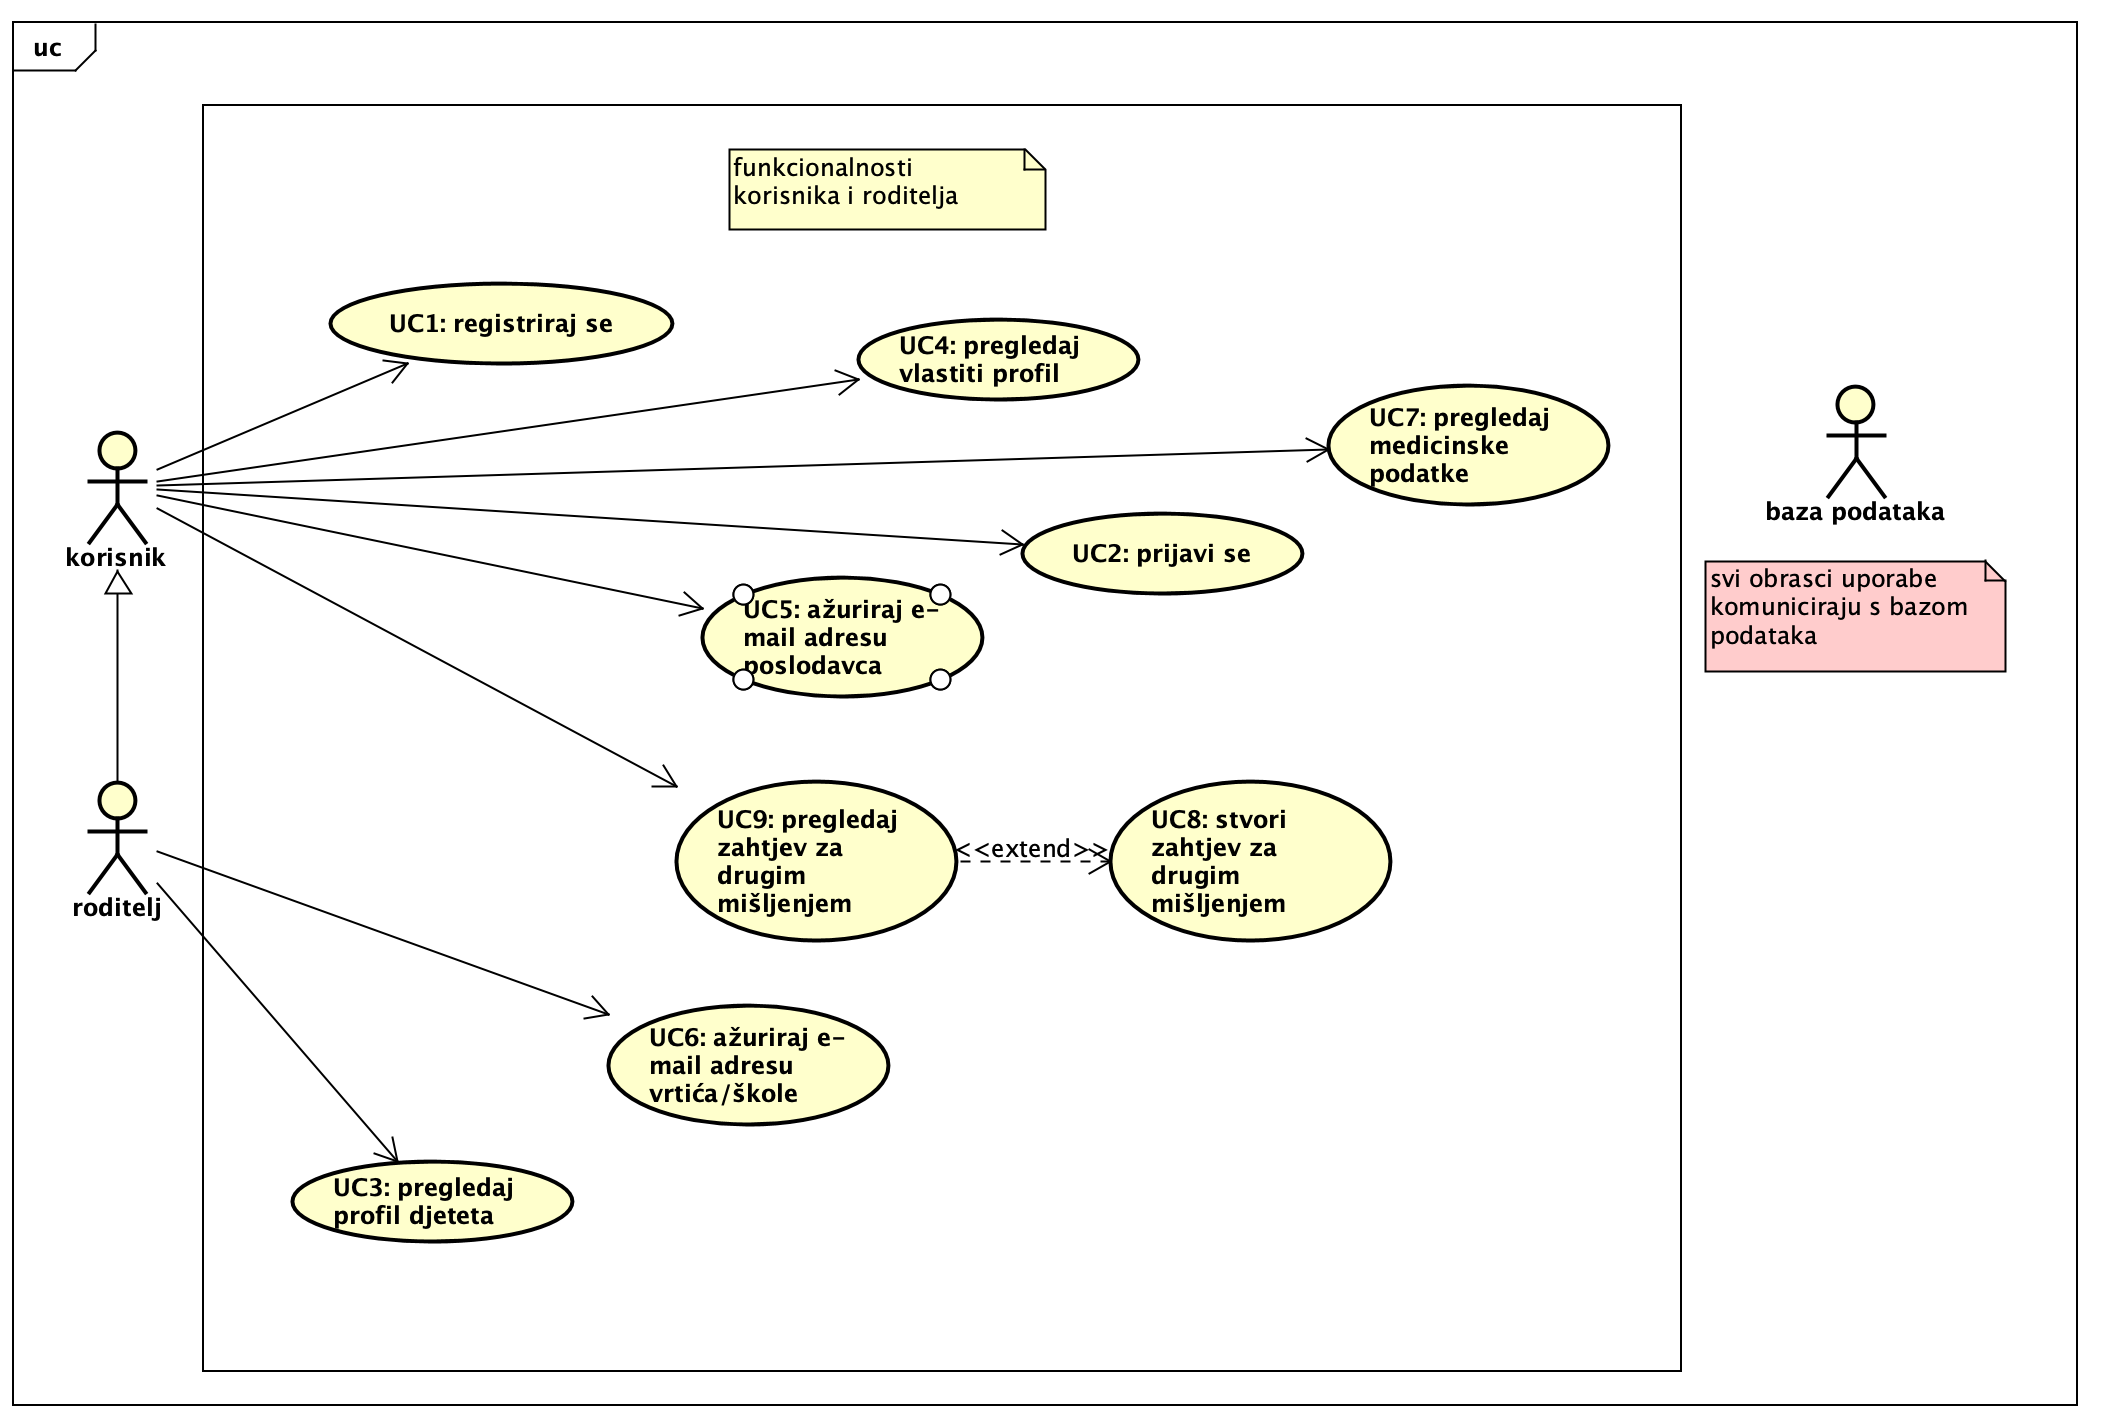
\includegraphics[width=\textwidth]{slike/uc_korisnik.png} 
						\caption{Dijagram obrasca uporabe, funkcionalnosti korisnika i roditelja}
						\label{fig:promjene2} 
					\end{figure}
					\begin{figure}[H]
						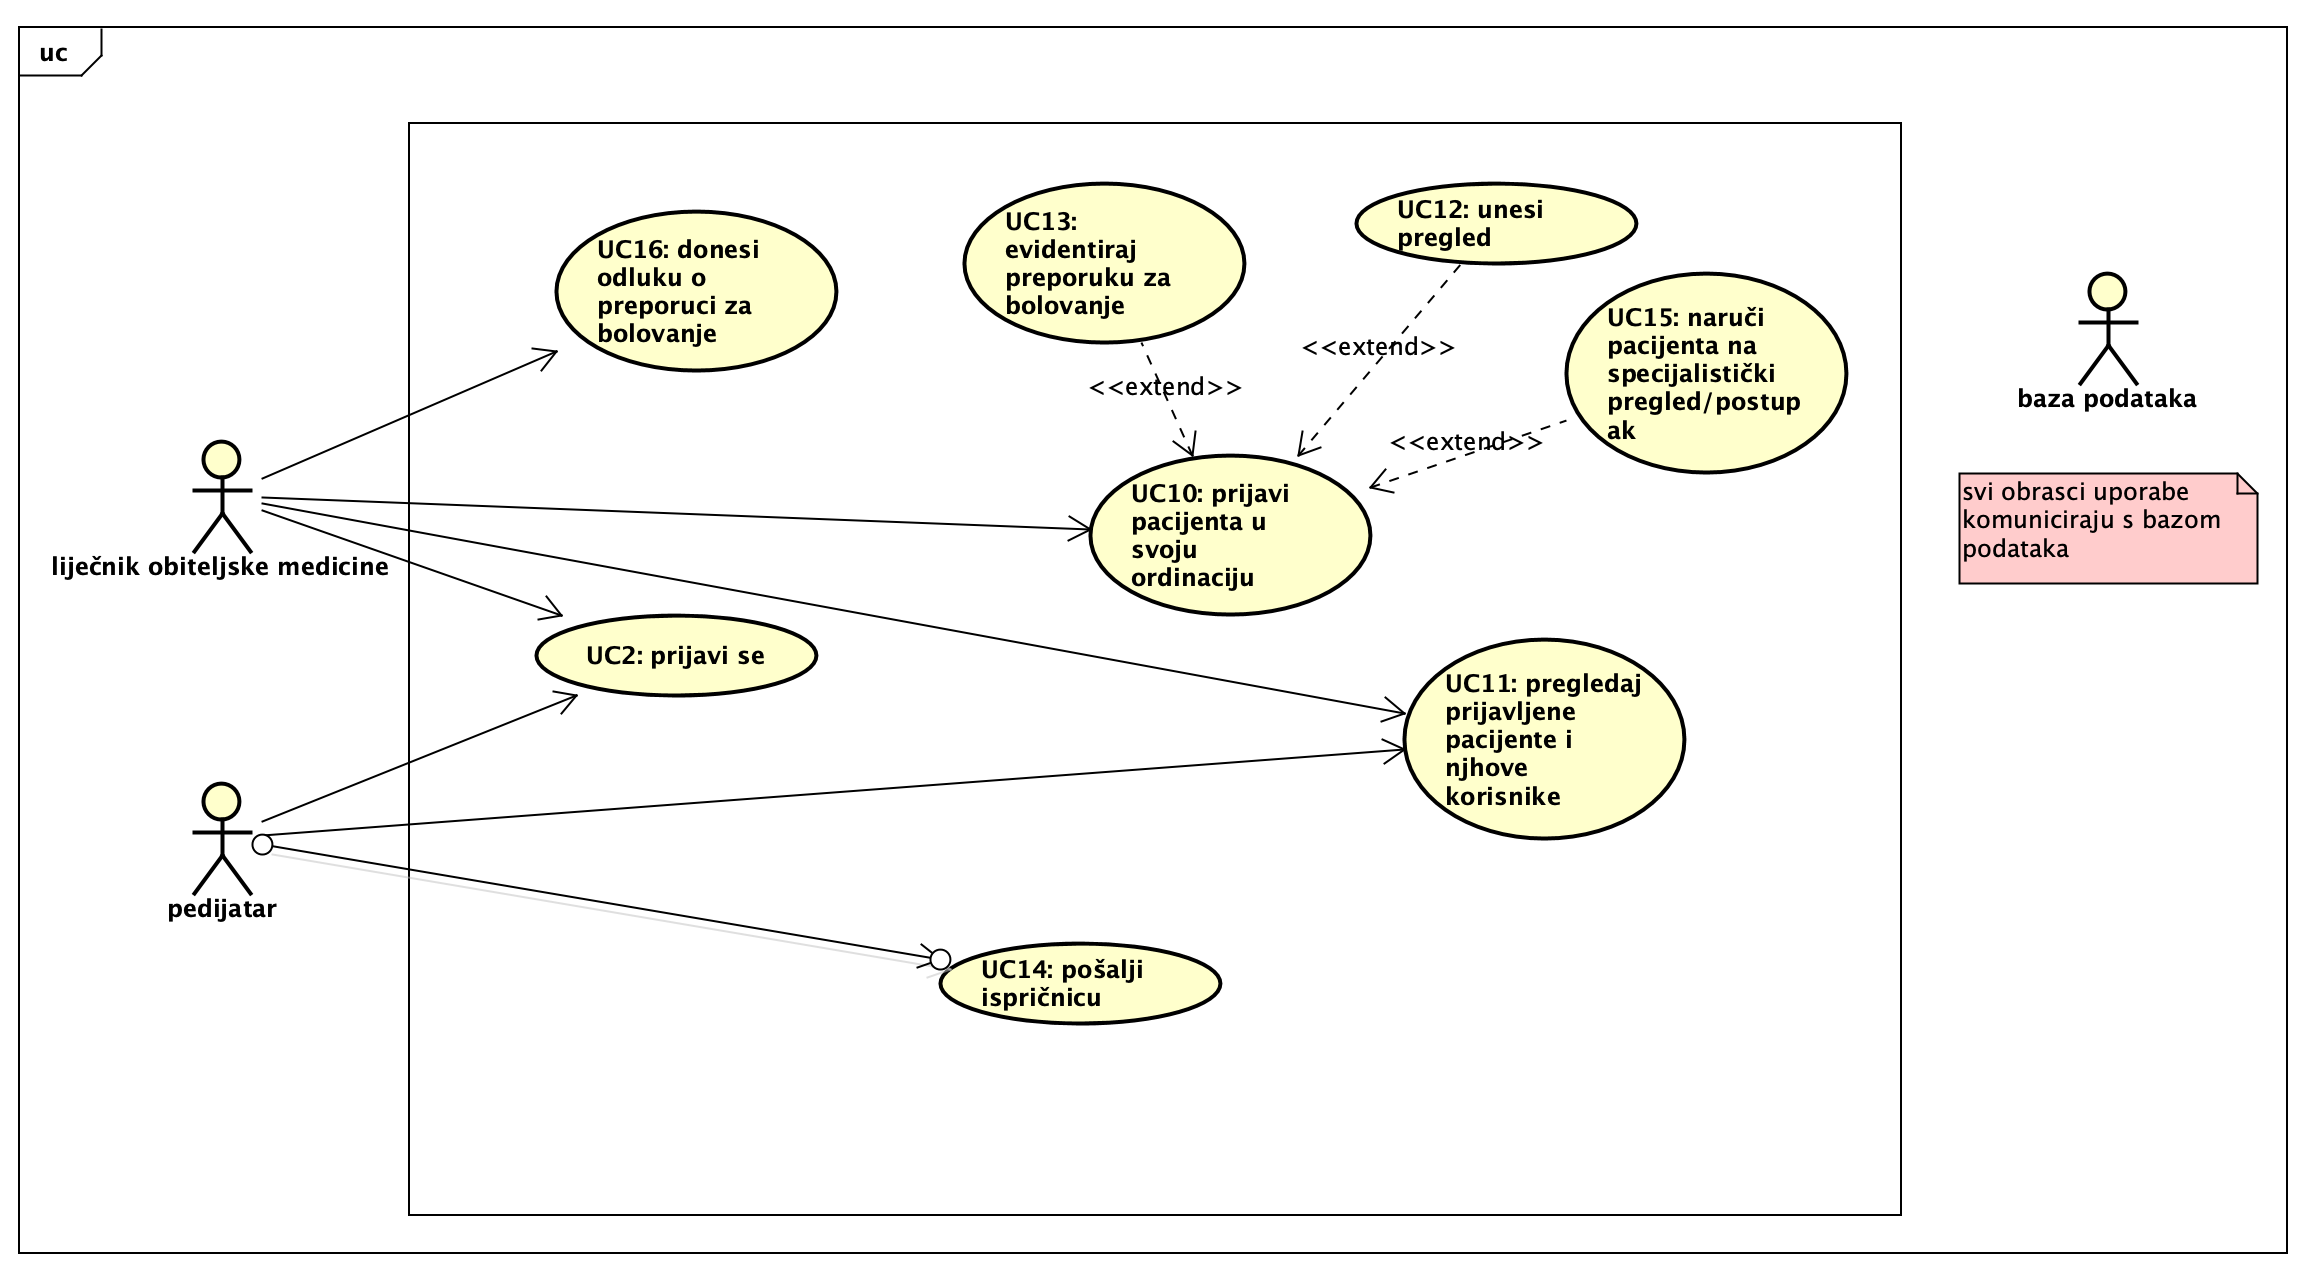
\includegraphics[width=\textwidth]{slike/uc_dr.png} 
						\caption{Dijagram obrasca uporabe, funkcionalnosti liječnika obiteljske medicine i pedijatra}
						\label{fig:promjene2} 
					\end{figure}
					\begin{figure}[H]
						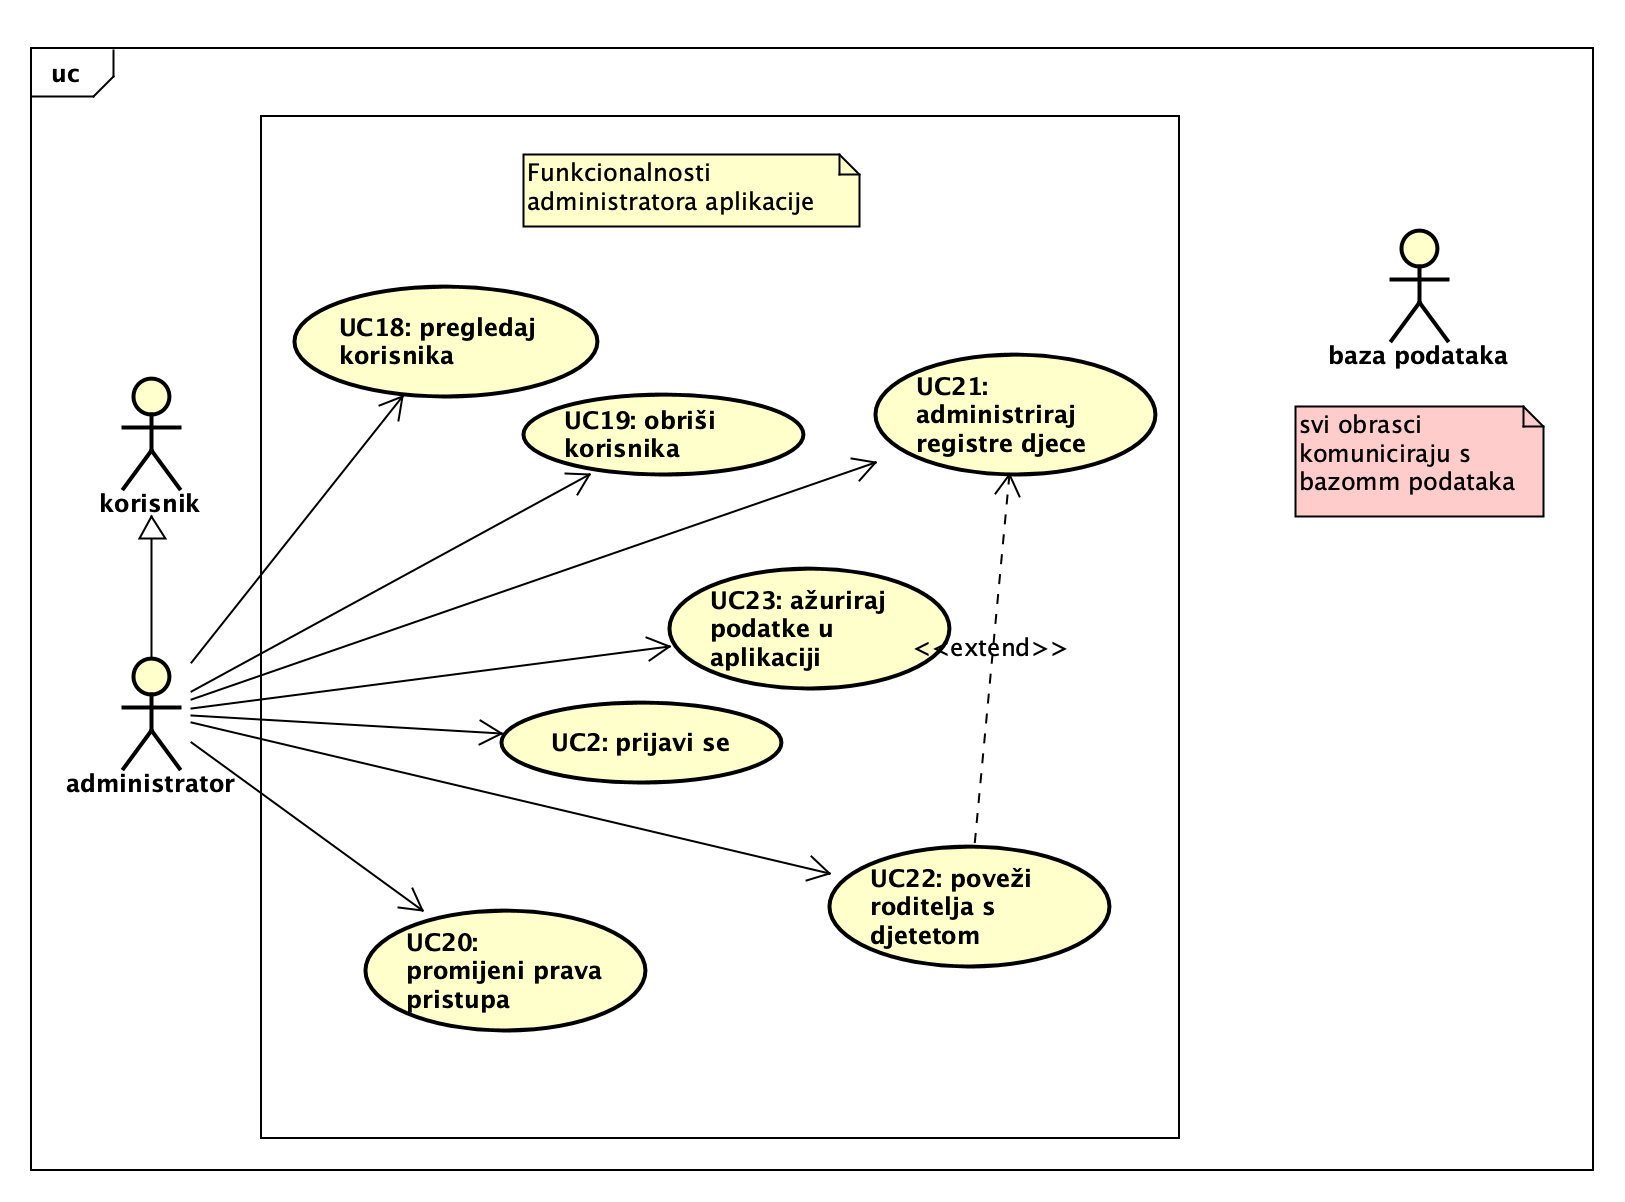
\includegraphics[width=\textwidth]{slike/uc_admin.png} 
						\caption{Dijagram obrasca uporabe, funkcionalnosti administratora}
						\label{fig:promjene2} 
					\end{figure}
				\eject		
				
			\subsection{Sekvencijski dijagrami}
				
				%dio 1. revizije
				
				%Nacrtati sekvencijske dijagrame koji modeliraju najvažnije dijelove sustava (max. 4 dijagrama). Uz svaki dijagram napisati detaljni opis dijagrama.
				\noindent\textbf{Obrazac uporabe UC8 - stvori zahtjev za drugim mišljenjem}
				Kroz proces potraživanja drugog mišljenja, korisnik inicira postupak odabirom opcije 
				'Zatraži drugo mišljenje'. Sustav odgovara otvaranjem modalnog okvira za unos zahtjeva, 
				gdje korisnik, u ovom slučaju roditelj, prenosi medicinski nalaz. Nakon toga, korisnik 
				bira specifičnog liječnika ili pedijatra čije drugo mišljenje želi dobiti i potvrđuje 
				zahtjev odabirom akcije 'Pošalji zahtjev'. Sustav potom provjerava i potvrđuje valjanost 
				unosa, prikazujući korisniku poruku o uspješnom slanju zahtjeva. U slučaju neispravno 
				popunjenog zahtjeva, sustav usmjerava korisnika na ponovni unos, osiguravajući točnost 
				informacija prije nastavka postupka. \\

				\begin{figure}[H]
						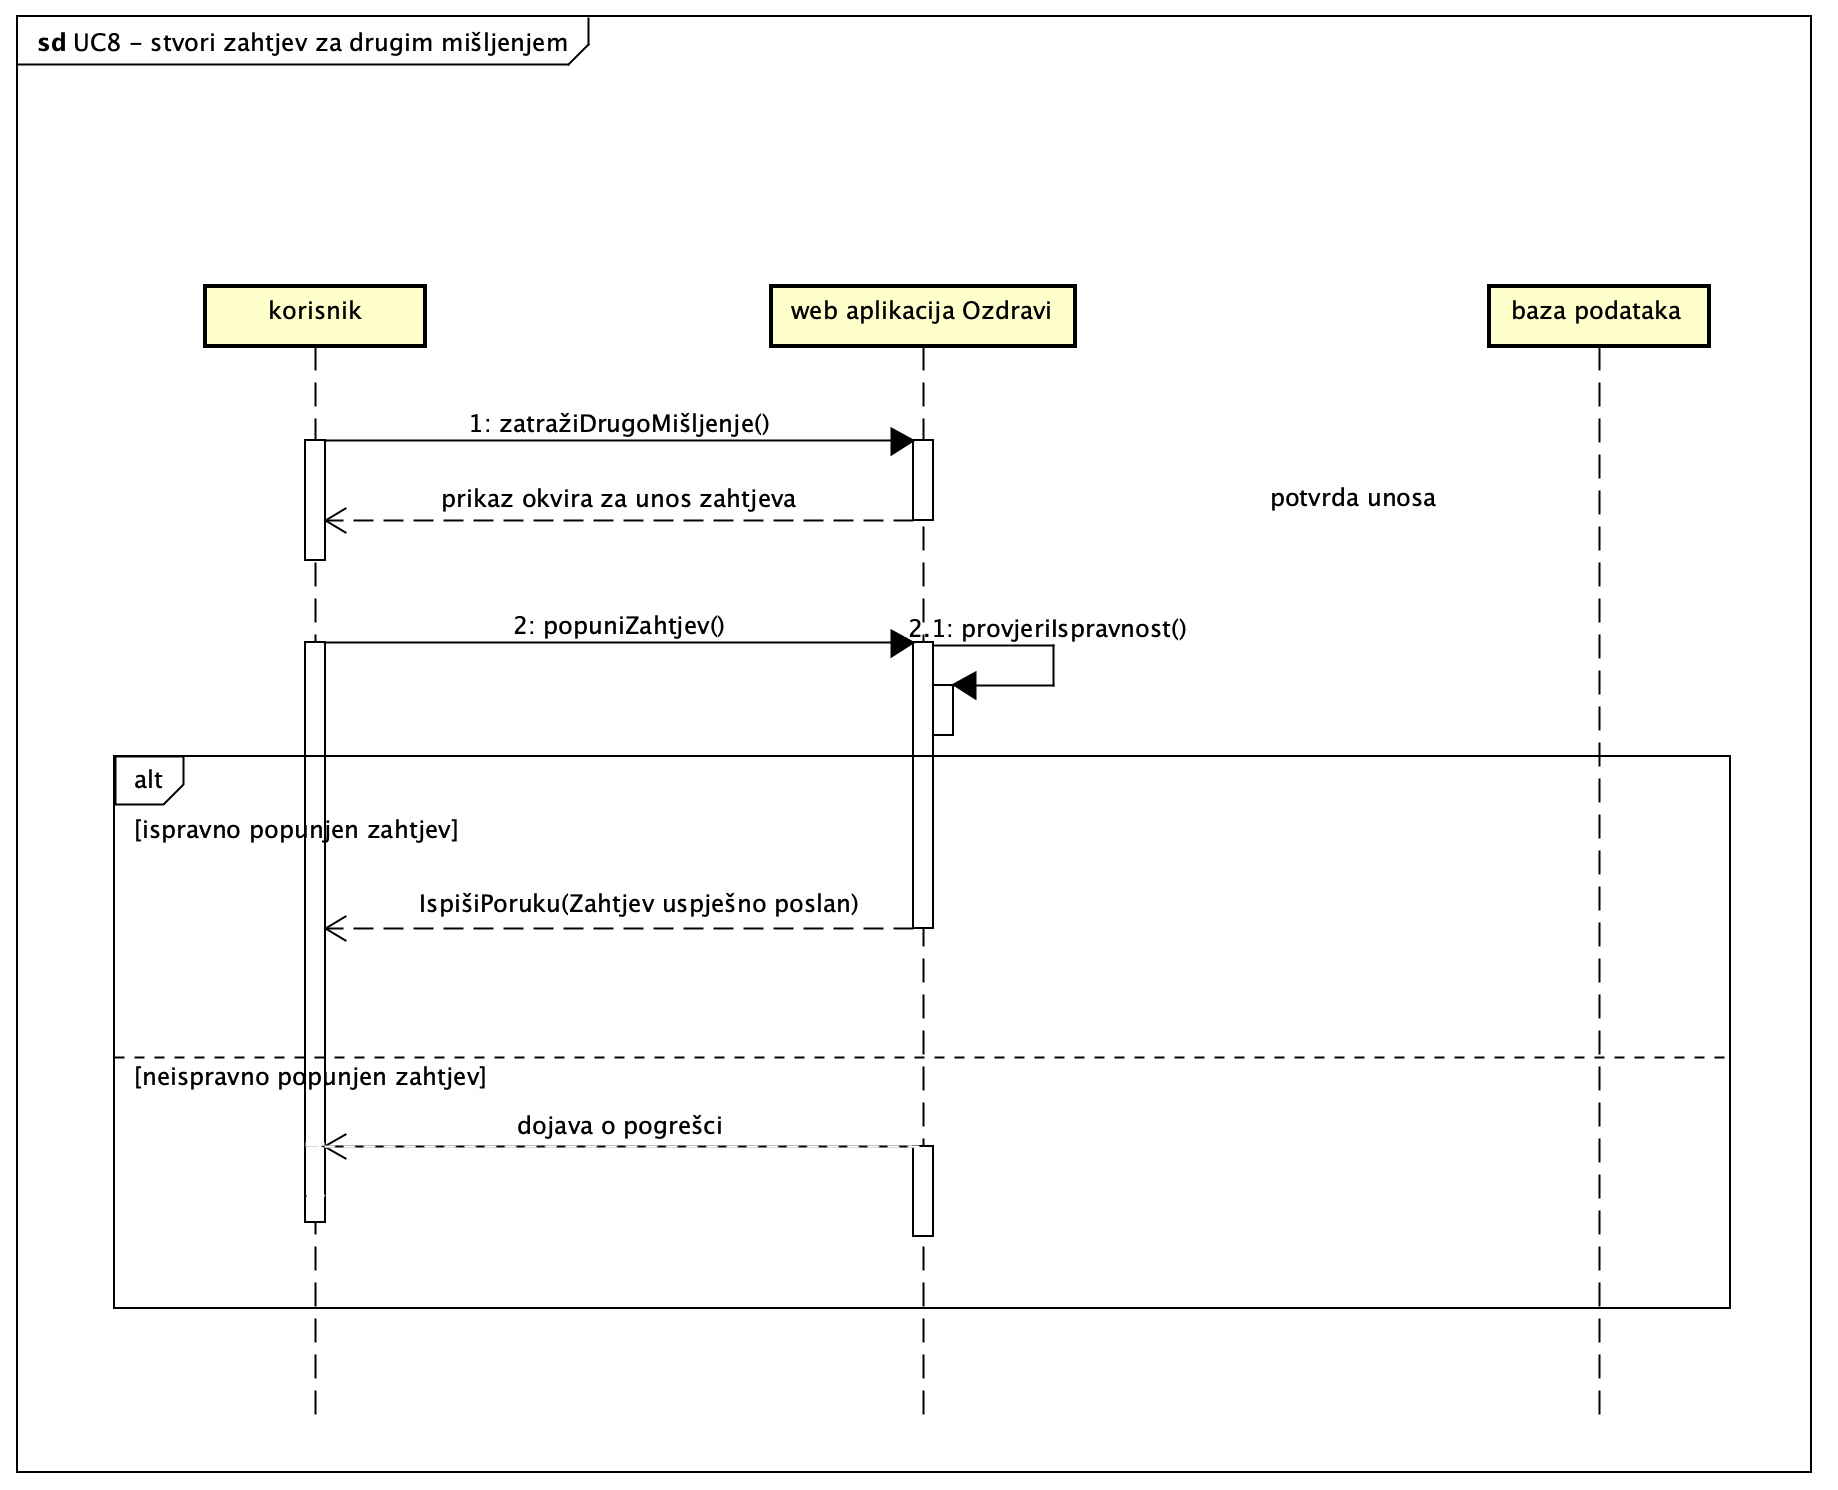
\includegraphics[width=\textwidth]{slike/sduc8.png} 
						\caption{Sekvencijski dijagram za UC8}
						\label{fig:promjene2} 
				\end{figure}
				\eject

				\noindent\textbf{Obrazac uporabe UC13 - evidentiraj preporuku za bolovanje}
				U postupku stvaranja nove preporuke za bolovanje, pedijatar započinje odabirom opcije 
				'Nova preporuka za bolovanje' s početne stranice. Sustav reagira prikazivanjem modalnog 
				okvira za unos preporuke za bolovanje. Pedijatar zatim odabire pregled na temelju kojeg 
				je potrebna preporuka za bolovanje i unosi relevantne podatke o preporuci. Kada završi 
				s unosom, pedijatar odabire opciju 'Unesi preporuku'. Sustav provjerava i potvrđuje 
				uspješan unos, nakon čega obavještava pedijatra o uspješnom dodavanju preporuke. \\

				\begin{figure}[H]
						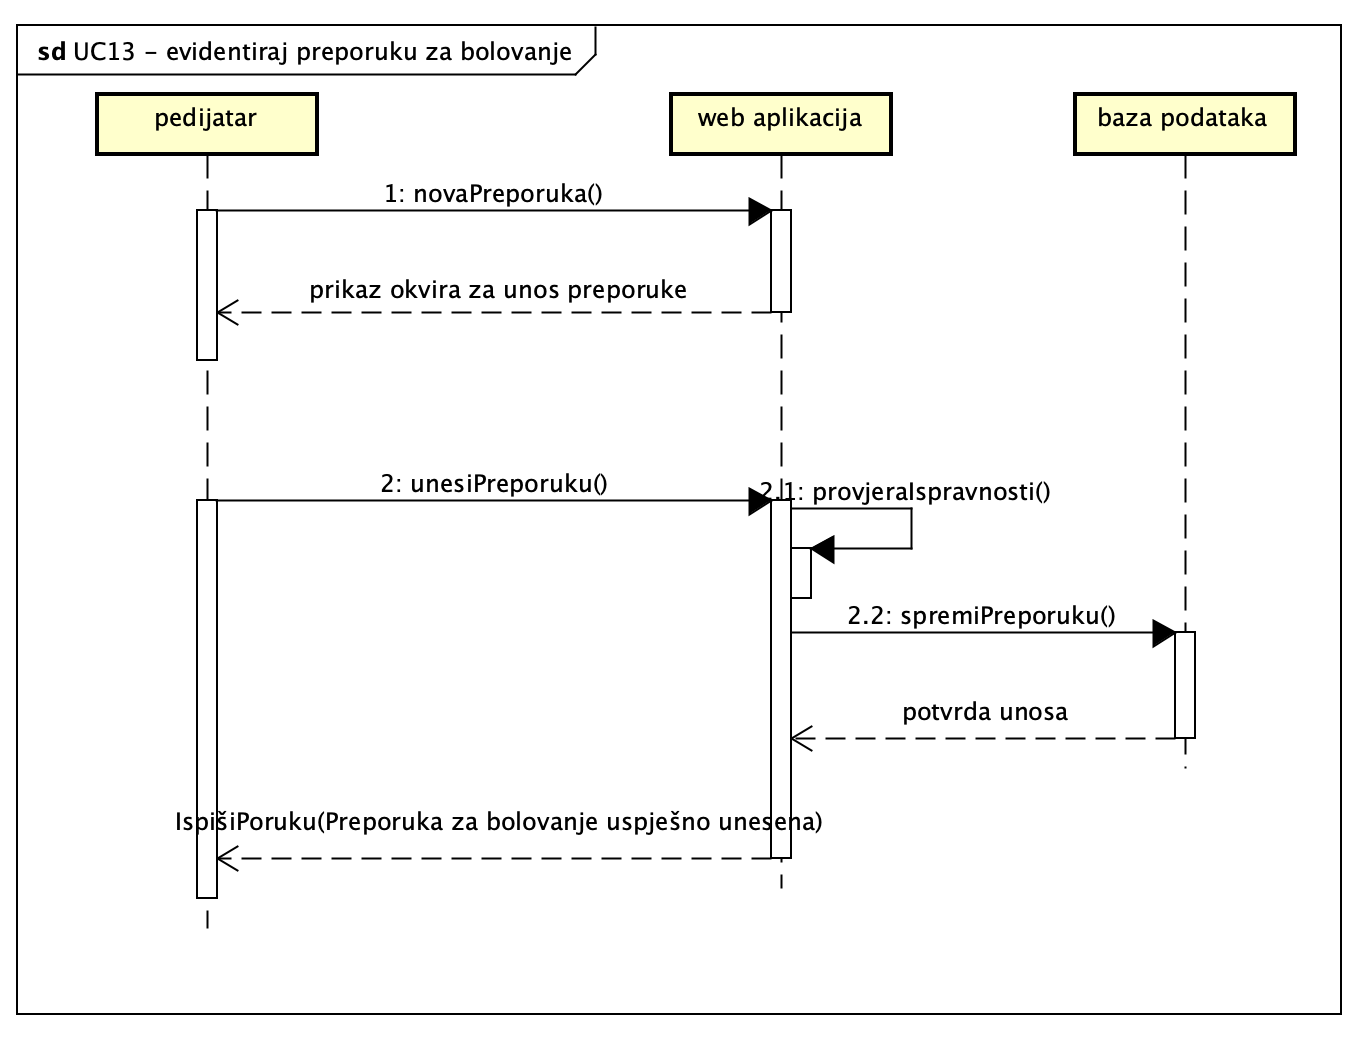
\includegraphics[width=\textwidth]{slike/sduc13.png} 
						\caption{Sekvencijski dijagram za UC13}
						\label{fig:promjene2} 
				\end{figure}
				\eject
				
				\noindent\textbf{Obrazac uporabe UC14 - evidentiraj preporuku za bolova}
				U procesu izdavanja nove ispričnice, pedijatar započinje odabirom opcije 'Nova ispričnica' 
				na početnoj stranici, što pokreće sustav da prikaže modalni ekran za unos ispričnice. 
				Pedijatar tada odabire pregled na temelju kojeg je potrebno poslati ispričnicu. Nakon 
				što popuni potrebne podatke, pedijatar odabire opciju 'Pošalji ispričnicu'. Sustav 
				izvršava provjeru i potvrđuje uspješan unos, nakon čega obavještava pedijatra da je 
				ispričnica uspješno poslana. U slučaju neispravnog popunjavanja ispričnice, sustav 
				prikazuje poruku o neispravnom unosu podataka, a pedijatar se vraća na ponovno 
				popunjavanje ispričnice, čime se scenarij nastavlja od koraka 4. \\

				\begin{figure}[H]
						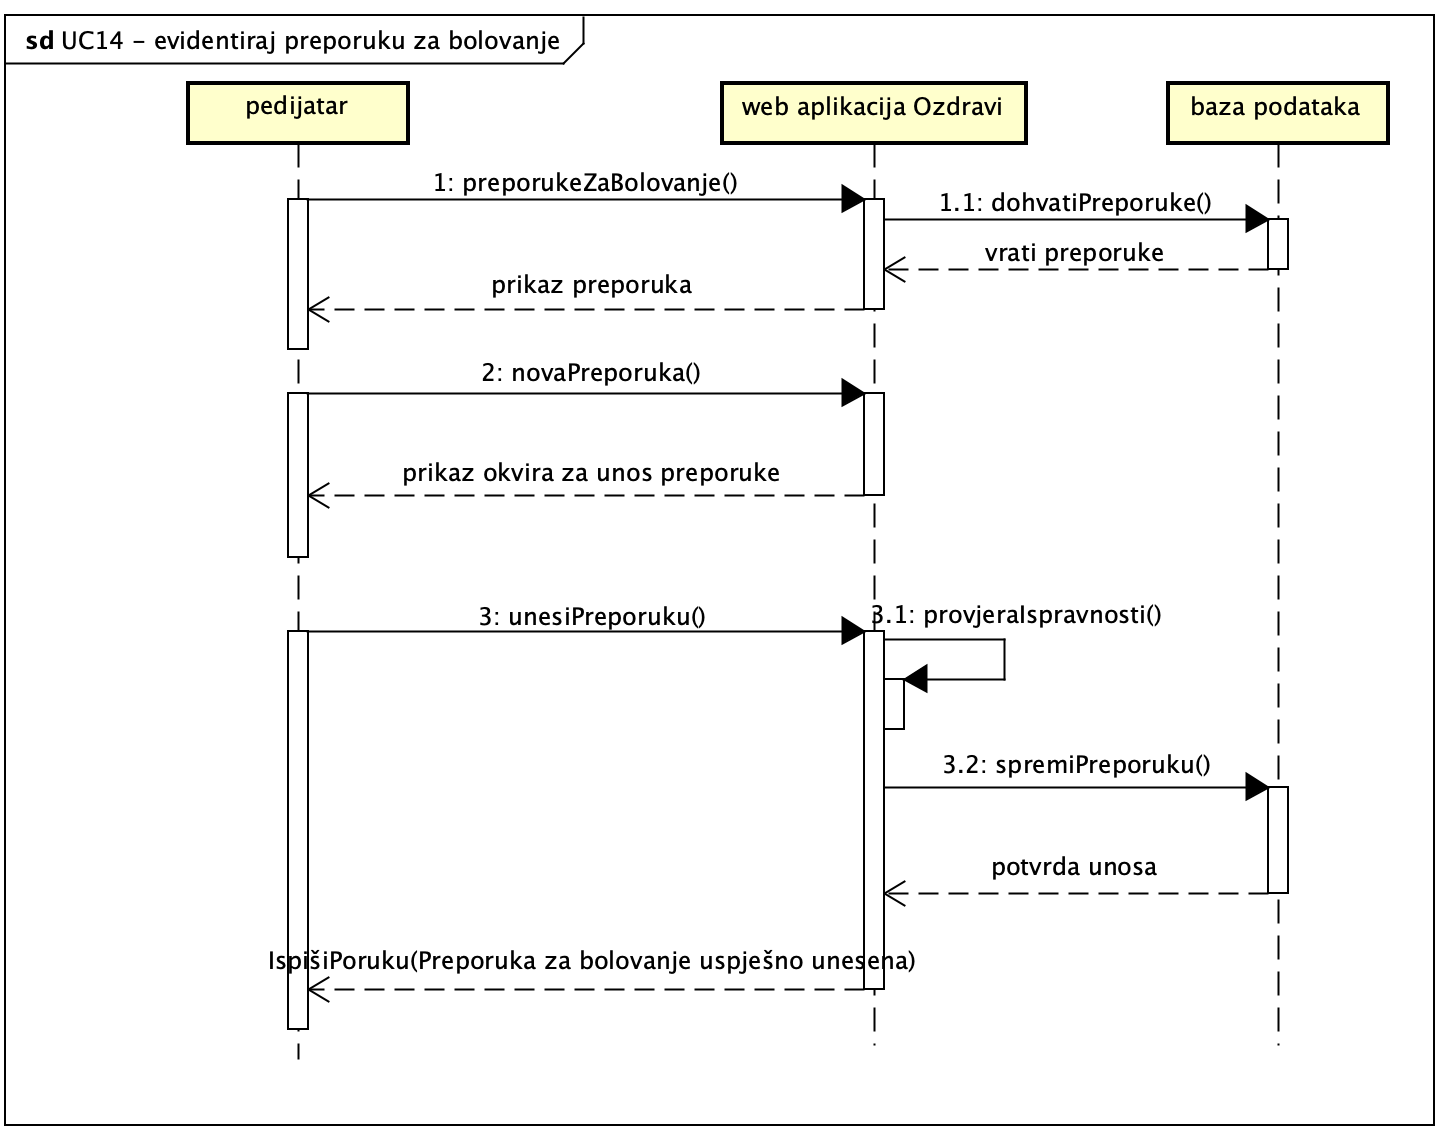
\includegraphics[width=\textwidth]{slike/sduc14.png} 
						\caption{Sekvencijski dijagram za UC14}
						\label{fig:promjene2} 
				\end{figure}

				\eject


	
		\section{Ostali zahtjevi}
			%dio 1. revizije
			 %Nefunkcionalni zahtjevi i zahtjevi domene primjene dopunjuju funkcionalne zahtjeve. Oni opisuju kako se sustav treba ponašati i koja ograničenja treba poštivati (performanse, korisničko iskustvo, pouzdanost, standardi kvalitete, sigurnost...). Primjeri takvih zahtjeva u Vašem projektu mogu biti: podržani jezici korisničkog sučelja, vrijeme odziva, najveći mogući podržani broj korisnika, podržane web/mobilne platforme, razina zaštite (protokoli komunikacije, kriptiranje...)... Svaki takav zahtjev potrebno je navesti u jednoj ili dvije rečenice.
			 \begin{packed_item}
				\item Sustav treba omogućiti rad više korisnika u stvarnom vremenu
				\item Sustav treba pružati brz odziv na korisničke zahtjeve
				\item Korisničko sučelje i sustav moraju podržavati hrvatsku abecedu (dijakritičke znakove) pri unosu i prikazu tekstualnog sadržaja
				\item Izvršavanje dijela programa u kojem se pristupa bazi podataka ne smije trajati duže od nekoliko sekundi
				\item Sustav treba biti implementiran kao web aplikacija koristeći objektno-orijentirane jezike
				\item Neispravno korištenje korisničkog sučelja ne smije narušiti funkcionalnost i rad sustava
				\item Sustav treba biti jednostavan za korištenje, sučelje treba biti intuitivno te se korisnici moraju znati koristiti sučeljem bez opširnih uputa
				\item Veza s bazom podataka mora biti kvalitetno zaštićena, brza i otporna na vanjske greške
				\item Pristup sustavu mora biti omogućen iz javne mreže pomoću HTTPS protokola
				\item Svi osjetljivi korisnički podaci, uključujući medicinske informacije, moraju biti kriptirani u 
				prijenosu i pohranjeni na način koji udovoljava standardima sigurnosti podataka u zdravstvenim aplikacijama
				\item Redovito automatsko izvođenje sigurnosnih kopija podataka s brzim i pouzdanim sustavom oporavka u slučaju neplaniranih događaja ili gubitka podataka
			 \end{packed_item}
			 	 
			 
	